\documentclass[tikz]{standalone}
\usepackage{pgfplots}
\pgfplotsset{compat=1.8}
\begin{document}
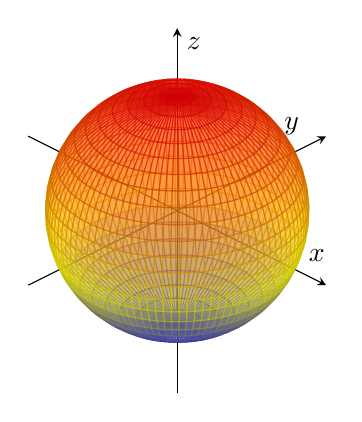
\begin{tikzpicture}
    \begin{axis}[%
        axis equal,
        width=10cm,
        height=10cm,
        axis lines = center,
        xlabel = {$x$},
        ylabel = {$y$},
        zlabel = {$z$},
        ticks=none,
        enlargelimits=0.3,
        view/h=45,
        scale uniformly strategy=units only,
    ]
    \addplot3[%
        opacity = 0.5,
        surf,
        z buffer = sort,
        samples = 50,
        variable = \u,
        variable y = \v,
        domain = 0:180,
        y domain = 0:360,
    ]
    ({cos(u)*sin(v)}, {sin(u)*sin(v)}, {cos(v)});

    \end{axis}
\end{tikzpicture}
\end{document}